\section{Лабораторная работа \textnumero{}1. Построение сеток в gmsh}

\subsection{Цель работы}

Метод конечных элементов (МКЭ) сводит дифференциальное уравнение
в частных производных к системе алгебраических уравнений, определённых
на дискретном разбиении области~--- \textit{сетке}. Качество этого
разбиения напрямую определяет точность и сходимость численного метода:
сильно вытянутые или «почти вырожденные» тетраэдры ухудшают обусловленность
матрицы жёсткости и порождают паразитные ошибки.

Цель работы~--- освоить построение таких разбиений с помощью библиотеки
\textbf{gmsh}: задание геометрии из аналитических примитивов, обработка
внешних STL-файлов и контроль качества элементов.

\subsection{Этап 1: Тор с полой внутренностью}

\subsubsection{Постановка задачи}

Требовалось построить тетраэдральную сетку тора с полой внутренней
полостью: не менее 3--4 тетраэдров должны умещаться в толщину стенки.

Это требование важно: если $h$ слишком велико, стенка
покрывается одним-двумя элементами и численный метод не разрешает
температурного (или механического) поля внутри неё. Поэтому по толщине
стенки нужно иметь хотя бы несколько элементов.

\subsubsection{Геометрия и булевы операции}

Полый тор строится в два шага. Сначала задаётся профиль (окружность
в плоскости $xOz$) четырьмя дугами с центром в точке $(R, 0, 0)$,
затем профиль вращается на $2\pi$ вокруг оси $z$:
\begin{equation}
  \mathbf{x}(\theta, \phi) =
  \bigl((R + r\cos\theta)\cos\phi,\;
         (R + r\cos\theta)\sin\phi,\;
         r\sin\theta\bigr),
  \quad \theta,\phi \in [0, 2\pi).
\end{equation}

Полость получается булевой операцией \texttt{cut}: из тела с параметрами
$(R=4,\, r=1)$ вычитается тело $(R=4,\, r=0.5)$. Оставшаяся оболочка
имеет толщину стенки $\Delta r = 0.5$. При характеристическом размере
элемента $h = 0.2$ в толщину укладывается $\lfloor 0.5/0.2 \rfloor + 1 = 3$--$4$
тетраэдра~--- ровно то, что требуется.

\newpage
\subsubsection{Реализация}

\begin{lstlisting}[language=C++, caption={Профиль и вращение тора}]
int CreateTorusProfile(const TorusParams &params) {
    double R = params.R, r = params.r;
    int p1 = gmsh::model::occ::addPoint(R + r, 0.0,  0.0);
    int p2 = gmsh::model::occ::addPoint(R,     0.0,  r  );
    int p3 = gmsh::model::occ::addPoint(R - r, 0.0,  0.0);
    int p4 = gmsh::model::occ::addPoint(R,     0.0, -r  );
    int pc = gmsh::model::occ::addPoint(R, 0.0, 0.0);
    int a1 = gmsh::model::occ::addCircleArc(p1, pc, p2);
    int a2 = gmsh::model::occ::addCircleArc(p2, pc, p3);
    int a3 = gmsh::model::occ::addCircleArc(p3, pc, p4);
    int a4 = gmsh::model::occ::addCircleArc(p4, pc, p1);
    return gmsh::model::occ::addCurveLoop({a1, a2, a3, a4});
}

// rotation around z-axis
gmsh::model::occ::revolve(
    {{2, surfTag}}, 0.0, 0.0, 0.0, 0.0, 0.0, 1.0, 2.0 * M_PI, out);
\end{lstlisting}

\begin{lstlisting}[language=C++, caption={Вычитаем полость тора}]
TorusParams outer{4.0, 1.0};  // outer span
TorusParams inner{4.0, 0.5};  // inner span
auto outerVol = CreateTorus(outer);
auto innerVol = CreateTorus(inner);
gmsh::model::occ::synchronize();
gmsh::model::occ::cut(cutObjects, toolObjects,
                      outMap, outMapTool, -1, true, true);
\end{lstlisting}

\subsubsection{Результат}

\begin{figure}[H]
  \centering
  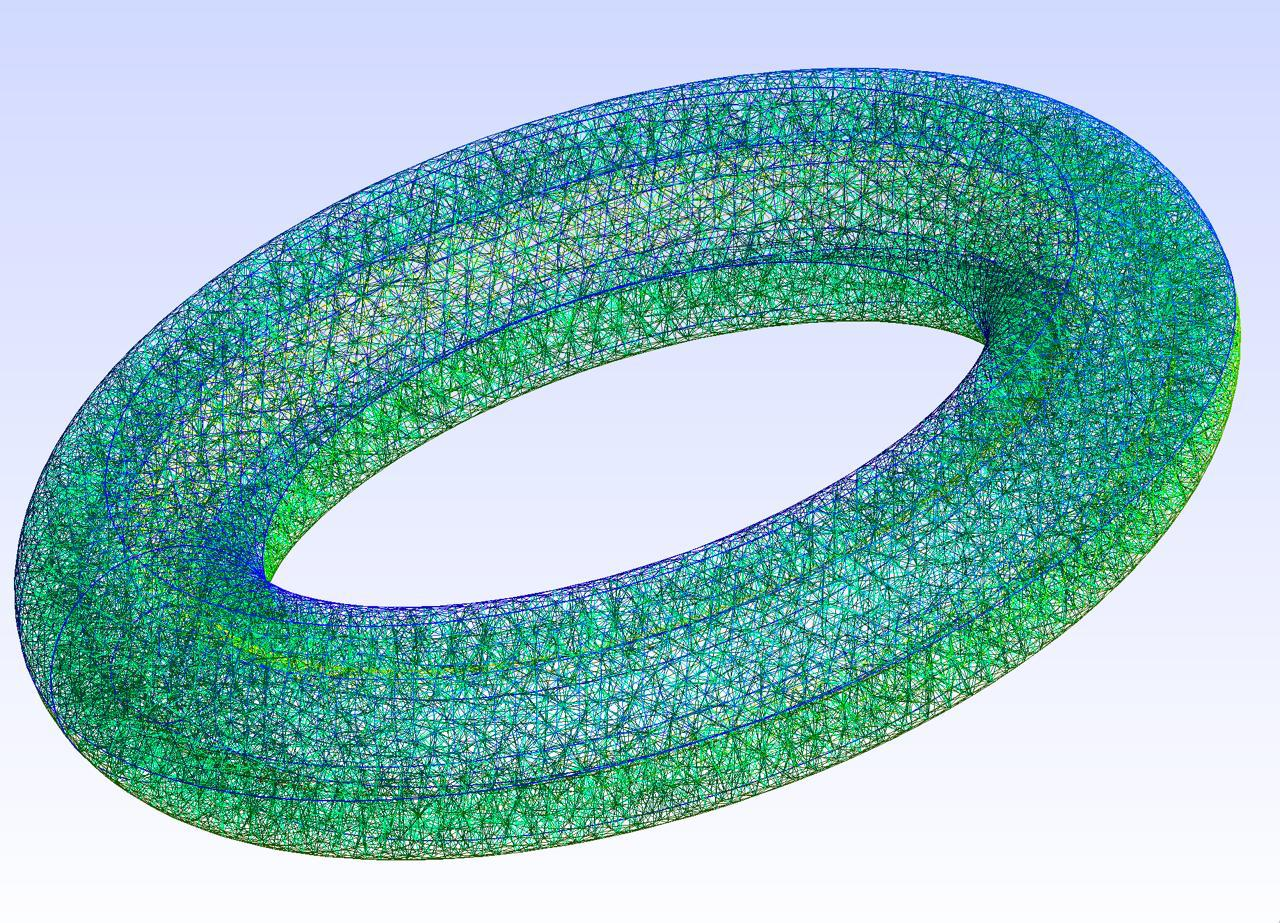
\includegraphics[width=0.75\linewidth]{img/lab1/torus1.png}
  \caption{Тетраэдральная сетка полого тора}
\end{figure}

Вид сбоку показывает, что в толщину стенки укладывается 3--4 элемента,
как и планировалось. Внутри полости элементы вытянутые, но при таком
соотношении размеров этого трудно избежать: радиус $R$ в 4 раза больше
толщины $\Delta r$, и при $h = 0.2$ по окружности получается примерно
20 элементов, а по толщине~--- 3--4.

\begin{figure}[H]
  \centering
  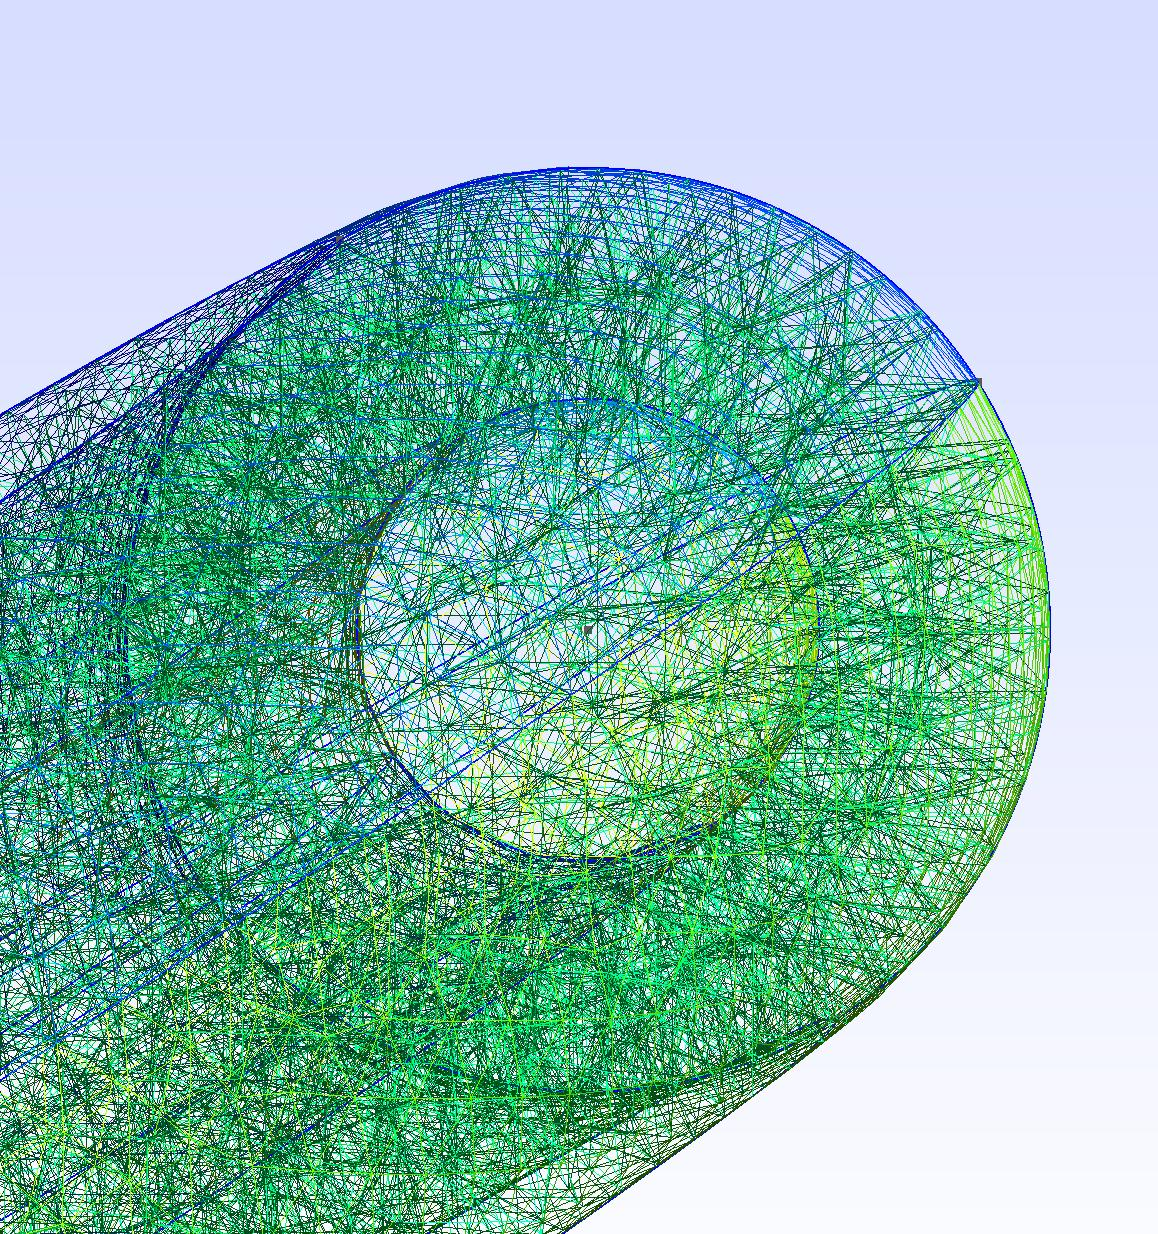
\includegraphics[width=0.5\linewidth]{img/lab1/torus2.png}
  \caption{Тетраэдральная сетка полого тора, вид сбоку}
\end{figure}

\subsection{Этап 2: Сетка в STL-объекте (карандаш)}

\subsubsection{Постановка задачи}

Граница реальных инженерных объектов часто задаётся не аналитически,
а триангулированной поверхностью~--- форматом STL. Это типичный вывод
систем 3D-моделирования и КТ-сканеров. Задача~--- построить объёмную
тетраэдральную сетку \textit{внутри} такого объекта.

\subsubsection{Проблема: STL описывает только поверхность}

STL содержит набор треугольных граней, но не несёт информации об объёме
и не имеет топологии (нет понятия «рёбра», «вершины» в смысле B-Rep).
Чтобы построить объёмную сетку, gmsh должен:
\begin{enumerate}
  \item Классифицировать грани по геометрическим признакам
        (выявить острые рёбра~--- границы патчей);
  \item Параметризовать поверхности~--- задать гладкую геометрию
        каждого патча, пригодную для проецирования узлов сетки;
  \item Сформировать замкнутый объём и заполнить его тетраэдрами.
\end{enumerate}

\subsubsection{Алгоритм классификации поверхностей}

Команда \texttt{classifySurfaces($\alpha$)} разделяет триангуляцию на
патчи: два соседних треугольника относятся к \textit{одному} патчу,
если двугранный угол между ними меньше $\alpha$. Острые рёбра
(угол $\ge \alpha$) становятся границами патчей. Для карандаша
$\alpha = 40^\circ$ отделяет грани ствола от граней заточки и торца.

После классификации \texttt{createGeometry} строит аналитическое
описание каждого патча через B-сплайны~--- это даёт правильные нормали
и возможность точно проецировать узлы на поверхность при генерации сетки.

\subsubsection{Реализация}

\begin{lstlisting}[language=C++, caption={Загрузка STL и построение объёмной сетки}]
gmsh::merge("pencil.stl");
gmsh::model::mesh::classifySurfaces(
    40 * M_PI / 180., true, false, 180 * M_PI / 180.);
gmsh::model::mesh::createGeometry();

vector<pair<int,int>> s;
gmsh::model::getEntities(s, 2);
vector<int> sl;
for (auto surf : s) sl.push_back(surf.second);

int l = gmsh::model::geo::addSurfaceLoop(sl);
gmsh::model::geo::addVolume({l});
gmsh::model::geo::synchronize();

gmsh::option::setNumber("Mesh.CharacteristicLengthMin", 2.0);
gmsh::option::setNumber("Mesh.CharacteristicLengthMax", 2.0);
gmsh::model::mesh::generate(3);
gmsh::write("pencil.msh");
\end{lstlisting}

\subsubsection{Результат}


\begin{figure}[H]
  \centering
  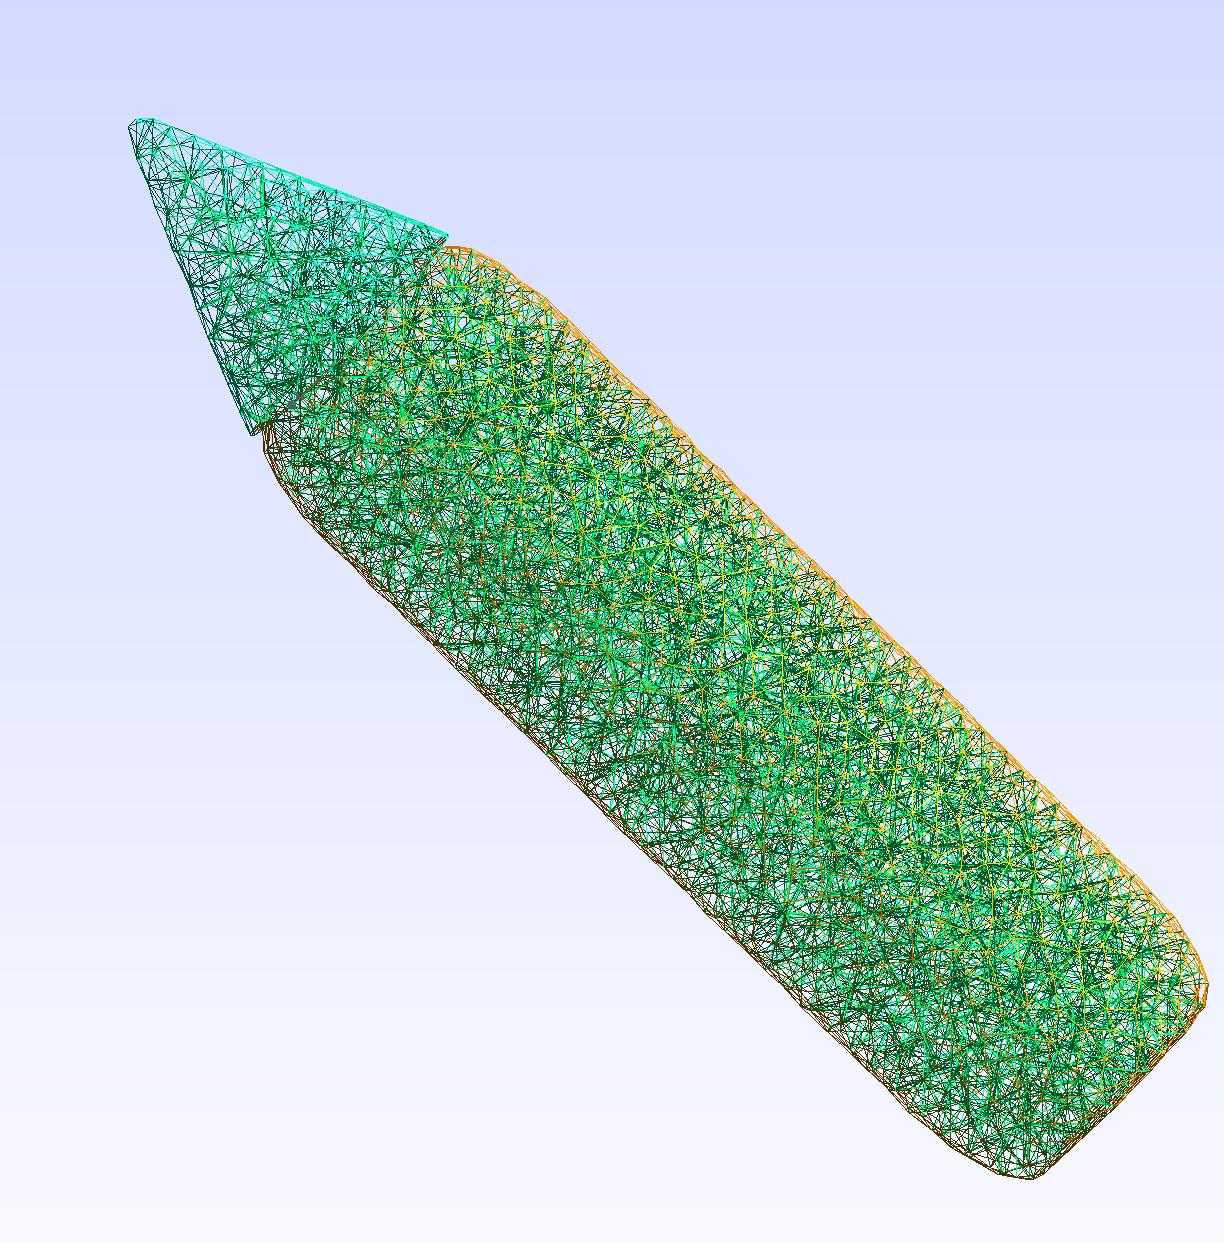
\includegraphics[width=0.75\linewidth]{img/lab1/pencil.png}
  \caption{Тетраэдральная сетка внутри STL-карандаша, $h = 2.0$.}
\end{figure}

\subsection{Выводы}

В работе освоены два принципиально разных подхода к построению
тетраэдральных сеток в gmsh.

\textbf{Конструктивная геометрия (CSG/OCC).} Область задаётся
аналитически~--- через примитивы и булевы операции.

\textbf{Восстановление из STL.} Область задаётся дискретной поверхностью
без аналитического описания. У сложных STL-моделей не всегда получается
автоматически выделить патчи, пригодные для генерации качественной
сетки. В таких случаях модель приходится вручную дорабатывать.
